\documentclass{resume}
\PassOptionsToPackage{russian, english}{babel}
\usepackage{babel}
\PassOptionsToPackage{utf8}{inputenc}
\usepackage{inputenc}
\usepackage{subfiles}
\usepackage{tikz}

\newcommand{\roundpic}[4][]{
  \tikz\node [circle, minimum width = #2,
    path picture = {
      \node [#1] at (path picture bounding box.center) {
        \includegraphics[width=#2]{#4}};
    }] {};}


\begin{document}

\fontfamily{ppl}\selectfont

\noindent
\begin{tabularx}{\linewidth}{@{}m{0.8\textwidth} m{0.2\textwidth}@{}}
{
    \Large{Nick Oliger} \newline
    \small{
        \clink{
            \href{mailto:naoliger@edu.hse.ru}{naoliger@edu.hse.ru} \textbf{·} 
            {\fontdimen2\font=0.75ex +7 963 122 71 45} 
            \textbf{·} 
            \href{}{tg:@polarnighty}
        } \newline
        Moscow, Russia
    }
} & 
{
    \hfill
    % \roundpic[yshift=-0.1cm]{4cm}{5cm}{images/portrait5.jpg}
    % 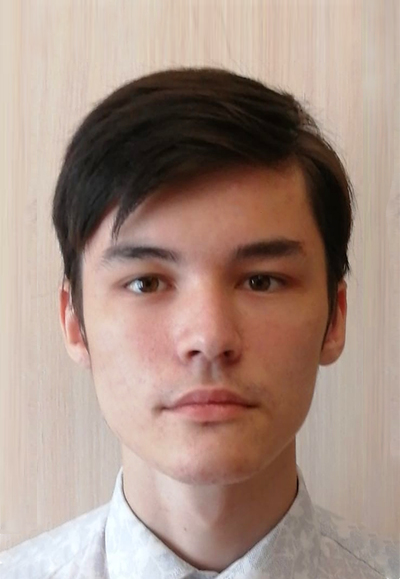
\includegraphics[width=3cm]{images/portrait.png} %
}
\end{tabularx}
\begin{center}
\begin{tabularx}{\linewidth}{@{}*{2}{X}@{}}
% left side %
{
    \csection{EDUCATION}{\small
        \begin{itemize}
            % item 1 %
            \item \frcontent{Higher education}{HSE, Faculty of Computer Science}{Applied Mathematics and Informatics}{2020 - Present}
            %\item \frcontent{Secondary education}{Gymnasium №26, math class \newline [Top 300 of Russian schools]}{}{2013 - 2020}
            
        \end{itemize}
    }
    \csection{WORKING \& TEACHING EXPERIENCE}{\small
        \begin{itemize}
            % item 1 %
            \item \frcontent{Yandex.Zen}{Intern at product development team}{Worked on backend using Java}{October 2021 - January 2022}
            % item 2 %
            \item \frcontent{Shkolkovo educational center}{Tutor}{Was responsible for organizing and checking math contests for 200+ students}{Summer 2020, Summer 2021}
            % item 3 %
            \item \frcontent{Shkolkovo educational center}{Mentor \& Tutor}{Was responsible for preparing 50+ students personally and 400+ students in total for math olympiads}{March 2020 - August 2022}
        \end{itemize}
    }
    \csection{SKILLS}{\small
        \begin{itemize}
            \item \textbf{Technologies} \newline
            {\footnotesize C++, Python, Java, Assembly, git, vim, \LaTeX}
            \item \textbf{Patterns \& Practices} \newline
            {\footnotesize Object Oriented Programming, Functional Programming, Distributed Systems, Machine Learning}
            \item \textbf{IDE} \newline
            {\footnotesize CLion, PyCharm, IntelliJIdea}
            \item \textbf{Languages} \newline
            {\footnotesize English: advanced | Russian: native}
        \end{itemize}
    }
} 
% end left side %
& 
% right side %
{
    \csection{AWARDS \& RECOGNITION}{\small
        \begin{itemize}
            % item 6 %
            \item \frcontent{Tinkoff scholarship holder}{Academic track}{}{2022-2023}
            % item 1 %
            \item \frcontent{Kurchatov, OMMO mathematical olympiads [2nd level]}{Awardee}{}{2020}
            % item 2 %
            \item \frcontent{Regional mathematical olympiad}{Awardee}{}{2019, 2018, 2017, 2016}
            % item 3 %
            \item \frcontent{MSU entering mathematical contest}{Score: 100/100}{}{2020}
	    % item 4 %
            \item \frcontent{Unified State Exam}{Math: 100, IT: 100, Russian: 98, English: 95}{}{2020}
            % item 5 %
            \item \frcontent{KFU english olympiad [2nd level]}{Awardee}{}{2019}
        \end{itemize}
    }
    \csection{PROJECTS}{\small
        \begin{itemize}
            \item \frcontent{Summer practice \clink{\href{https://github.com/NickMadeIt/hse_weather_bot }{[HSE Weather Bot]}}}{Telegram bot showing current weather forecast using open API}{}{Python, TeleBot, git}
        \end{itemize}
    }
    %\csection{OTHER HIGHLIGHTS}{\small
    %    \begin{itemize}
    %        \item {\footnotesize Used to be committing to IT startup for soulmates from Yandex.Taxi using %SQLAlchemy, Flask.}
    %    \end{itemize}
    %}
    \csection{HOBBIES \& INTERESTS}{\small
        \vspace{0.1cm}
        \begin{tabularx}{\linewidth}{@{}*{4}{>{\centering\arraybackslash}X}@{}}
            {\centering
            
\includegraphics[width=0.8cm]{images/light-bulb-in-a-circle-with-small-circles.png}
            } &
            {\centering
            
\includegraphics[width=0.8cm]{images/soccer.png}
            } & 
            {\centering
            
\includegraphics[width=0.8cm]{images/small-duck.png}
            } &
            {\centering
            
\includegraphics[width=0.8cm]{images/reception-desk.png}
            } \\
            {\footnotesize Learning languages} & {\footnotesize Board games} & {\footnotesize Swimming} & {\footnotesize Teaching}
        \end{tabularx}
    }
}
\end{tabularx}
\end{center}
\end{document}
